% Options for packages loaded elsewhere
\PassOptionsToPackage{unicode}{hyperref}
\PassOptionsToPackage{hyphens}{url}
%
\documentclass[
  a4paper,
]{article}
\usepackage{amsmath,amssymb}
\usepackage{iftex}
\ifPDFTeX
  \usepackage[T1]{fontenc}
  \usepackage[utf8]{inputenc}
  \usepackage{textcomp} % provide euro and other symbols
\else % if luatex or xetex
  \usepackage{unicode-math} % this also loads fontspec
  \defaultfontfeatures{Scale=MatchLowercase}
  \defaultfontfeatures[\rmfamily]{Ligatures=TeX,Scale=1}
\fi
\usepackage{lmodern}
\ifPDFTeX\else
  % xetex/luatex font selection
  \setmainfont[]{Helvetica}
\fi
% Use upquote if available, for straight quotes in verbatim environments
\IfFileExists{upquote.sty}{\usepackage{upquote}}{}
\IfFileExists{microtype.sty}{% use microtype if available
  \usepackage[]{microtype}
  \UseMicrotypeSet[protrusion]{basicmath} % disable protrusion for tt fonts
}{}
\makeatletter
\@ifundefined{KOMAClassName}{% if non-KOMA class
  \IfFileExists{parskip.sty}{%
    \usepackage{parskip}
  }{% else
    \setlength{\parindent}{0pt}
    \setlength{\parskip}{6pt plus 2pt minus 1pt}}
}{% if KOMA class
  \KOMAoptions{parskip=half}}
\makeatother
\usepackage{xcolor}
\usepackage[margin=1in]{geometry}
\usepackage{graphicx}
\makeatletter
\def\maxwidth{\ifdim\Gin@nat@width>\linewidth\linewidth\else\Gin@nat@width\fi}
\def\maxheight{\ifdim\Gin@nat@height>\textheight\textheight\else\Gin@nat@height\fi}
\makeatother
% Scale images if necessary, so that they will not overflow the page
% margins by default, and it is still possible to overwrite the defaults
% using explicit options in \includegraphics[width, height, ...]{}
\setkeys{Gin}{width=\maxwidth,height=\maxheight,keepaspectratio}
% Set default figure placement to htbp
\makeatletter
\def\fps@figure{htbp}
\makeatother
\setlength{\emergencystretch}{3em} % prevent overfull lines
\providecommand{\tightlist}{%
  \setlength{\itemsep}{0pt}\setlength{\parskip}{0pt}}
\setcounter{secnumdepth}{-\maxdimen} % remove section numbering
\usepackage{titling}
\pretitle{\begin{flushleft}}
\posttitle{\end{flushleft}}
\usepackage{booktabs}
\usepackage{longtable}
\usepackage{float}
\floatplacement{figure}{H}
\usepackage{colortbl}
\usepackage{pdflscape}
\usepackage{tabu}
\usepackage{makecell}
\usepackage{xcolor}
\usepackage{soul}
\usepackage{caption}
\usepackage[singlelinecheck=false]{caption}
\usepackage[font={small,bf}]{caption}
\usepackage{multirow}
\usepackage{array}
\usepackage{booktabs}
\usepackage{longtable}
\usepackage{array}
\usepackage{multirow}
\usepackage{wrapfig}
\usepackage{float}
\usepackage{colortbl}
\usepackage{pdflscape}
\usepackage{tabu}
\usepackage{threeparttable}
\usepackage{threeparttablex}
\usepackage[normalem]{ulem}
\usepackage{makecell}
\usepackage{xcolor}
\ifLuaTeX
  \usepackage{selnolig}  % disable illegal ligatures
\fi
\usepackage{bookmark}
\IfFileExists{xurl.sty}{\usepackage{xurl}}{} % add URL line breaks if available
\urlstyle{same}
\hypersetup{
  hidelinks,
  pdfcreator={LaTeX via pandoc}}

\title{\vspace{-1.5cm} \begin{LARGE} WGS Quality Control Report \end{LARGE}}
\author{}
\date{\vspace{-2.5em}}

\begin{document}
\maketitle

\normalsize Batch Name: 2024-04-07

\normalsize Experiment Name: 24ARS\_EMR\_LG788

\fontsize{7}{8}
\selectfont
\captionsetup[table]{labelformat=empty}
\renewcommand{\arraystretch}{1.2}

\begin{longtable}[t]{>{\centering\arraybackslash}p{1cm}>{\centering\arraybackslash}p{2cm}>{\centering\arraybackslash}p{1.5cm}>{\centering\arraybackslash}p{5.25cm}>{\centering\arraybackslash}p{5.25cm}}
\toprule
\multicolumn{1}{>{\centering\arraybackslash}p{1cm}}{\cellcolor[HTML]{D4D4D4}{\textbf{Isolate No.}}} & \multicolumn{1}{>{\centering\arraybackslash}p{2cm}}{\cellcolor[HTML]{D4D4D4}{\textbf{Sample ID}}} & \multicolumn{1}{>{\centering\arraybackslash}p{1.5cm}}{\cellcolor[HTML]{D4D4D4}{\textbf{Description}}} & \multicolumn{1}{>{\centering\arraybackslash}p{5.25cm}}{\cellcolor[HTML]{D4D4D4}{\textbf{ARSRL}}} & \multicolumn{1}{>{\centering\arraybackslash}p{5.25cm}}{\cellcolor[HTML]{D4D4D4}{\textbf{WGS}}}\\
\midrule
1 & 23ARS\_VSM0511 & SAL68 & Salmonella species & \cellcolor{white}{Salmonella enterica subsp. enterica serovar Enteritidis}\\
2 & 24ARS\_BRH0014 & EMR142\_2 & Pseudomonas aeruginosa & \cellcolor{white}{Pseudomonas aeruginosa}\\
3 & 24ARS\_BRT0017 & EMR141\_2 & Pseudomonas aeruginosa & \cellcolor{white}{Pseudomonas aeruginosa}\\
4 & 24ARS\_CRH0017 & EMR146 & Escherichia coli & \cellcolor{white}{Escherichia coli}\\
5 & 24ARS\_CRH0030 & EMR148 & Klebsiella pneumoniae & \cellcolor{white}{Klebsiella quasipneumoniae}\\
\addlinespace
6 & 24ARS\_DMC0098 & EMR149 & Klebsiella pneumoniae & \cellcolor{white}{Klebsiella pneumoniae}\\
7 & 24ARS\_DMC0102 & EMR157 & Pseudomonas aeruginosa & \cellcolor{white}{Pseudomonas aeruginosa}\\
8 & 24ARS\_EVR0011 & EMR155 & Pseudomonas aeruginosa & \cellcolor{white}{Pseudomonas aeruginosa}\\
9 & 24ARS\_EVR0017 & EMR158 & Pseudomonas aeruginosa & \cellcolor{white}{Pseudomonas aeruginosa}\\
10 & 24ARS\_GMH0029 & EMR145 & Klebsiella pneumoniae & \cellcolor{white}{Klebsiella pneumoniae}\\
\addlinespace
11 & 24ARS\_JLM0018 & EMR143 & Klebsiella pneumoniae & \cellcolor{white}{Klebsiella pneumoniae}\\
12 & 24ARS\_JLM0020 & EMR144 & Klebsiella pneumoniae & \cellcolor{white}{Klebsiella quasipneumoniae}\\
13 & 24ARS\_NKI0048 & EMR147 & Escherichia coli & \cellcolor{white}{Escherichia coli}\\
14 & 24ARS\_NKI0050 & EMR150 & Klebsiella pneumoniae & \cellcolor{white}{Klebsiella pneumoniae}\\
15 & 24ARS\_NKI0051 & EMR151 & Klebsiella pneumoniae & \cellcolor{white}{Klebsiella pneumoniae}\\
\addlinespace
16 & 24ARS\_SLH0030 & EMR154 & Pseudomonas aeruginosa & \cellcolor{white}{Pseudomonas aeruginosa}\\
17 & 24ARS\_STU0024 & EMR152 & Klebsiella pneumoniae & \cellcolor{white}{Klebsiella pneumoniae}\\
18 & 24ARS\_STU0027 & EMR153 & Acinetobacter baumannii & \cellcolor{white}{Acinetobacter pittii}\\
\cellcolor[HTML]{FFA77F}{19} & \cellcolor[HTML]{FFA77F}{24ARS\_ZMC0002} & \cellcolor[HTML]{FFA77F}{EMR156} & \cellcolor[HTML]{FFA77F}{Pseudomonas aeruginosa} & \cellcolor[HTML]{FFA77F}{Pseudomonas aeruginosa}\\
20 & UTP\_BL\_006 & tricycle & Escherichia coli & \cellcolor{white}{Escherichia coli}\\
\addlinespace
21 & UTP\_ST\_031 & tricycle & Escherichia coli & \cellcolor{white}{Escherichia coli}\\
\bottomrule
\end{longtable}

\tiny Legend: \begingroup\fontsize{4}{6}\selectfont

\begin{tabular}{|>{\centering\arraybackslash}p{1cm}|>{\centering\arraybackslash}p{1cm}|>{\centering\arraybackslash}p{1cm}|>{\centering\arraybackslash}p{3cm}|>{\centering\arraybackslash}p{2cm}|}

\cellcolor{white}{PASS} & \cellcolor[HTML]{FFA77F}{WARNING} & \cellcolor[HTML]{FD7979}{FAILURE} & \textcolor{blue}{EXCEEDS THRESHOLD METRIC/S} & \cellcolor{yellow}{NON-CONCORDANT}\\

\end{tabular}
\endgroup{}
\fontsize{7}{8}
\selectfont
\captionsetup[table]{labelformat=empty}
\renewcommand{\arraystretch}{1.2}

\begin{tabular}{>{\centering\arraybackslash}p{3cm}>{\centering\arraybackslash}p{3cm}>{\centering\arraybackslash}p{2cm}>{\centering\arraybackslash}p{7cm}}
\toprule
\multicolumn{4}{l}{\textbf{Sample excluded in the analysis}} \\
\cmidrule(l{3pt}r{3pt}){1-4}
\multicolumn{1}{>{\centering\arraybackslash}p{3cm}}{\cellcolor[HTML]{D4D4D4}{\textbf{Sample ID}}} & \multicolumn{1}{>{\centering\arraybackslash}p{3cm}}{\cellcolor[HTML]{D4D4D4}{\textbf{Description}}} & \multicolumn{1}{>{\centering\arraybackslash}p{2cm}}{\cellcolor[HTML]{D4D4D4}{\textbf{Index reads}}} & \multicolumn{1}{>{\centering\arraybackslash}p{7cm}}{\cellcolor[HTML]{D4D4D4}{\textbf{Remarks}}}\\
\midrule
24ARS\_NKI0053 & EMR159 & 0.8429 & low read count\\
\bottomrule
\end{tabular}

\(\\\)

\fontsize{7}{8}
\selectfont
\captionsetup[table]{labelformat=empty}
\renewcommand{\arraystretch}{1.2}

\begin{longtable}[t]{>{\centering\arraybackslash}p{1cm}>{\centering\arraybackslash}p{3cm}>{\centering\arraybackslash}p{2cm}>{\centering\arraybackslash}p{2cm}>{\centering\arraybackslash}p{2cm}>{\centering\arraybackslash}p{2cm}>{\centering\arraybackslash}p{2cm}}
\toprule
\multicolumn{1}{>{\centering\arraybackslash}p{1cm}}{\cellcolor[HTML]{D4D4D4}{\textbf{Isolate No.}}} & \multicolumn{1}{>{\centering\arraybackslash}p{3cm}}{\cellcolor[HTML]{D4D4D4}{\textbf{Sample ID}}} & \multicolumn{1}{>{\centering\arraybackslash}p{2cm}}{\cellcolor[HTML]{D4D4D4}{\textbf{Contamination}}} & \multicolumn{1}{>{\centering\arraybackslash}p{2cm}}{\cellcolor[HTML]{D4D4D4}{\textbf{Contigs}}} & \multicolumn{1}{>{\centering\arraybackslash}p{2cm}}{\cellcolor[HTML]{D4D4D4}{\textbf{GC Percent}}} & \multicolumn{1}{>{\centering\arraybackslash}p{2cm}}{\cellcolor[HTML]{D4D4D4}{\textbf{N50}}} & \multicolumn{1}{>{\centering\arraybackslash}p{2cm}}{\cellcolor[HTML]{D4D4D4}{\textbf{Total Length}}}\\
\midrule
1 & 23ARS\_VSM0511 & \textcolor{black}{0} & \textcolor{black}{24} & 52.13 & \textcolor{black}{478941} & 4700439\\
2 & 24ARS\_BRH0014 & \textcolor{black}{0} & \textcolor{black}{84} & 65.97 & \textcolor{black}{247991} & 6878546\\
3 & 24ARS\_BRT0017 & \textcolor{black}{0} & \textcolor{black}{122} & 65.33 & \textcolor{black}{220628} & 7348540\\
4 & 24ARS\_CRH0017 & \textcolor{black}{0} & \textcolor{black}{127} & 50.53 & \textcolor{black}{136602} & 5373741\\
5 & 24ARS\_CRH0030 & \textcolor{black}{0} & \textcolor{black}{39} & 57.75 & \textcolor{black}{801312} & 5379490\\
\addlinespace
6 & 24ARS\_DMC0098 & \textcolor{black}{0} & \textcolor{black}{44} & 57.19 & \textcolor{black}{479099} & 5405179\\
7 & 24ARS\_DMC0102 & \textcolor{black}{0} & \textcolor{black}{51} & 66.32 & \textcolor{black}{488628} & 6482852\\
8 & 24ARS\_EVR0011 & \textcolor{black}{0} & \textcolor{black}{47} & 66.47 & \textcolor{black}{407140} & 6291421\\
9 & 24ARS\_EVR0017 & \textcolor{black}{0} & \textcolor{black}{131} & 66.36 & \textcolor{black}{151006} & 6423637\\
10 & 24ARS\_GMH0029 & \textcolor{black}{0} & \textcolor{black}{110} & 56.65 & \textcolor{black}{172819} & 5772594\\
\addlinespace
11 & 24ARS\_JLM0018 & \textcolor{black}{0} & \textcolor{black}{95} & 56.79 & \textcolor{black}{394359} & 5742923\\
12 & 24ARS\_JLM0020 & \textcolor{black}{0} & \textcolor{black}{77} & 57.65 & \textcolor{black}{229344} & 5512178\\
13 & 24ARS\_NKI0048 & \textcolor{black}{0} & \textcolor{black}{93} & 50.83 & \textcolor{black}{320376} & 5148168\\
14 & 24ARS\_NKI0050 & \textcolor{black}{0} & \textcolor{black}{55} & 57.20 & \textcolor{black}{236088} & 5425644\\
15 & 24ARS\_NKI0051 & \textcolor{black}{0} & \textcolor{black}{81} & 56.82 & \textcolor{black}{238924} & 5595191\\
\addlinespace
16 & 24ARS\_SLH0030 & \textcolor{black}{0} & \textcolor{black}{99} & 65.94 & \textcolor{black}{361062} & 6937344\\
17 & 24ARS\_STU0024 & \textcolor{black}{0} & \textcolor{black}{55} & 57.13 & \textcolor{black}{303929} & 5493891\\
18 & 24ARS\_STU0027 & \textcolor{black}{0} & \textcolor{black}{17} & 38.58 & \textcolor{black}{519454} & 3995354\\
\cellcolor[HTML]{FFA77F}{19} & \cellcolor[HTML]{FFA77F}{24ARS\_ZMC0002} & \cellcolor[HTML]{FFA77F}{\textcolor{black}{0}} & \cellcolor[HTML]{FFA77F}{\textcolor{black}{89}} & \cellcolor[HTML]{FFA77F}{66.46} & \cellcolor[HTML]{FFA77F}{\textcolor{black}{197528}} & \cellcolor[HTML]{FFA77F}{6319285}\\
20 & UTP\_BL\_006 & \textcolor{black}{0} & \textcolor{black}{44} & 50.61 & \textcolor{black}{279880} & 4940847\\
\addlinespace
21 & UTP\_ST\_031 & \textcolor{black}{0} & \textcolor{black}{109} & 50.42 & \textcolor{black}{166206} & 5380880\\
\bottomrule
\end{longtable}

\tiny Legend: \begingroup\fontsize{4}{6}\selectfont

\begin{tabular}{|>{\centering\arraybackslash}p{1cm}|>{\centering\arraybackslash}p{1cm}|>{\centering\arraybackslash}p{1cm}|>{\centering\arraybackslash}p{2.5cm}|>{\centering\arraybackslash}p{8cm}|}

\cellcolor{white}{PASS} & \cellcolor[HTML]{FFA77F}{WARNING} & \cellcolor[HTML]{FD7979}{FAILURE} & \textcolor{blue}{EXCEEDS THRESHOLD METRIC/S} & *Isolates were tagged with warning due to uncertain results  of species identification using bactinspector or sequence identification levels.\\

\end{tabular}
\endgroup{}

\fontsize{7}{8}
\selectfont
\captionsetup[table]{labelformat=empty}
\renewcommand{\arraystretch}{1.2}

\begin{longtable}[l]{>{\centering\arraybackslash}p{3cm}>{\centering\arraybackslash}p{12cm}}
\toprule
\multicolumn{2}{l}{\textbf{List of samples above/below QC threshold metrics}} \\
\cmidrule(l{3pt}r{3pt}){1-2}
\cellcolor[HTML]{D4D4D4}{\textbf{Sample ID}} & \cellcolor[HTML]{D4D4D4}{\textbf{Remarks}}\\
\midrule
 & No QC failures found.\\
\bottomrule
\end{longtable}

\fontsize{7}{8}
\selectfont
\captionsetup[table]{labelformat=empty}
\renewcommand{\arraystretch}{1.2}

\begin{longtable}[l]{>{\raggedright\arraybackslash}p{8cm}c}
\toprule
\cellcolor[HTML]{D4D4D4}{\textbf{WGS\_ID}} & \cellcolor[HTML]{D4D4D4}{\textbf{Number}}\\
\midrule
Pseudomonas aeruginosa & 7\\
Klebsiella pneumoniae & 6\\
Escherichia coli & 4\\
Klebsiella quasipneumoniae & 2\\
Acinetobacter pittii & 1\\
\addlinespace
Salmonella enterica subsp. enterica serovar Enteritidis & 1\\
\bottomrule
\end{longtable}

\begin{itemize}
\item
  \(\color{red}6\) distinct species were identified among
  \(\color{red}21\) isolates.
\item
  \(\color{red}95.24\) \% (n=20) of the isolates passed the QC, while
  \(\color{red}4.76\) \% (n=1) were tagged with warning.
\item
  Concordance between ARSRL and WGS species report was
  \(\color{red}100.00\) \%. \(\\\)
\end{itemize}

\subsubsection{GRAPHS}\label{graphs}

\fontsize{7}{8}
\selectfont
\captionsetup[table]{labelformat=empty}
\renewcommand{\arraystretch}{1.2}

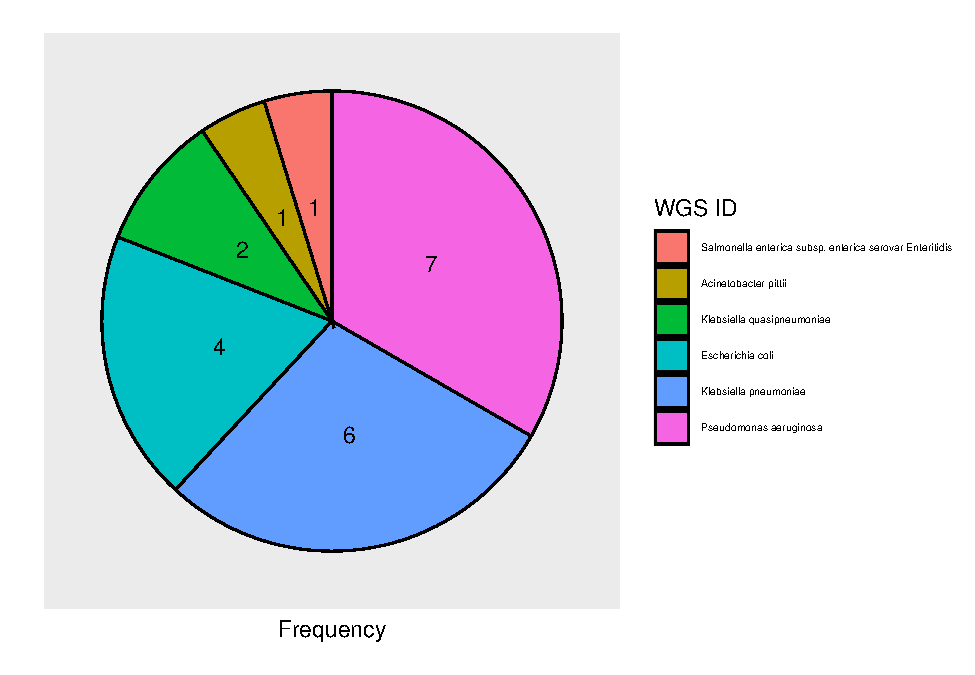
\includegraphics{qualifyr_report_2024-04-07_files/figure-latex/pie_chart-1.pdf}

\subsubsection{Result Classification}\label{result-classification}

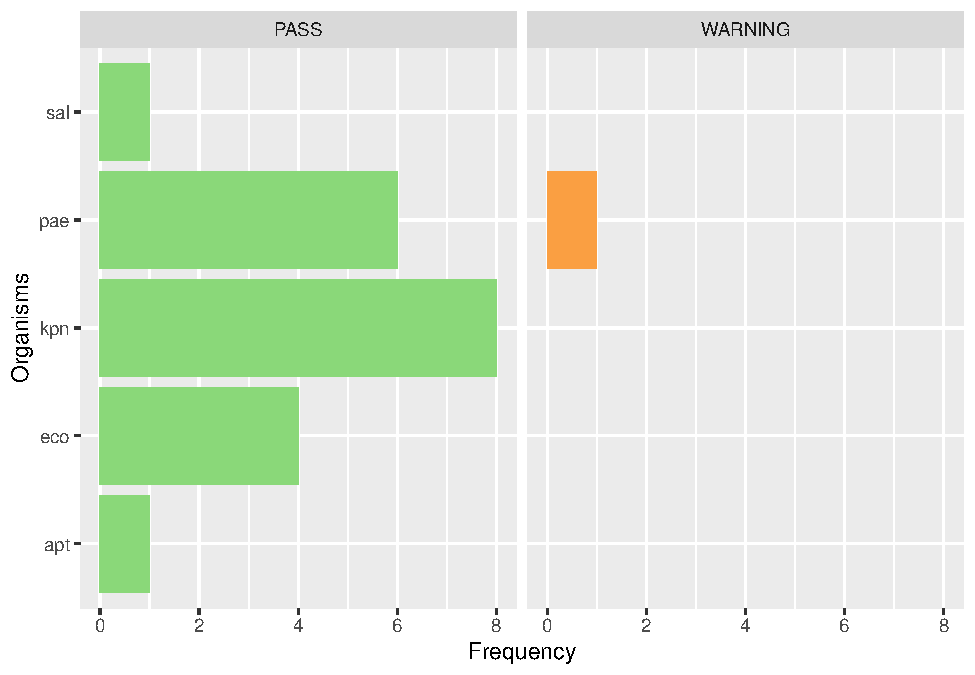
\includegraphics{qualifyr_report_2024-04-07_files/figure-latex/organism results-1.pdf}

\subsubsection{Number of contigs}\label{number-of-contigs}

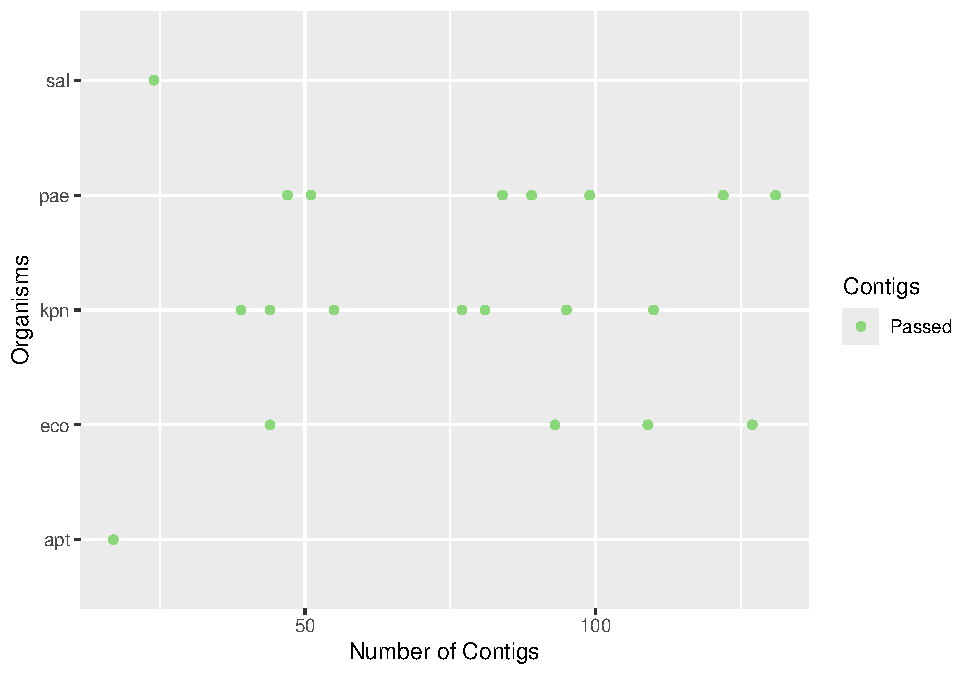
\includegraphics{qualifyr_report_2024-04-07_files/figure-latex/unnamed-chunk-1-1.pdf}

\subsubsection{N50 Value}\label{n50-value}

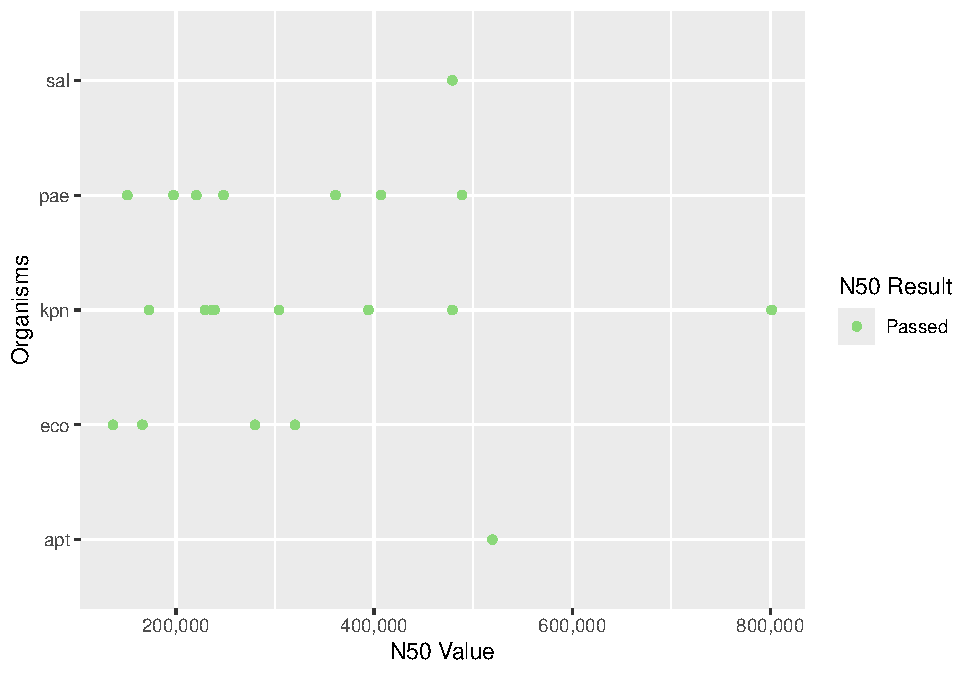
\includegraphics{qualifyr_report_2024-04-07_files/figure-latex/n50_result -1.pdf}

\subsubsection{Total Length}\label{total-length}

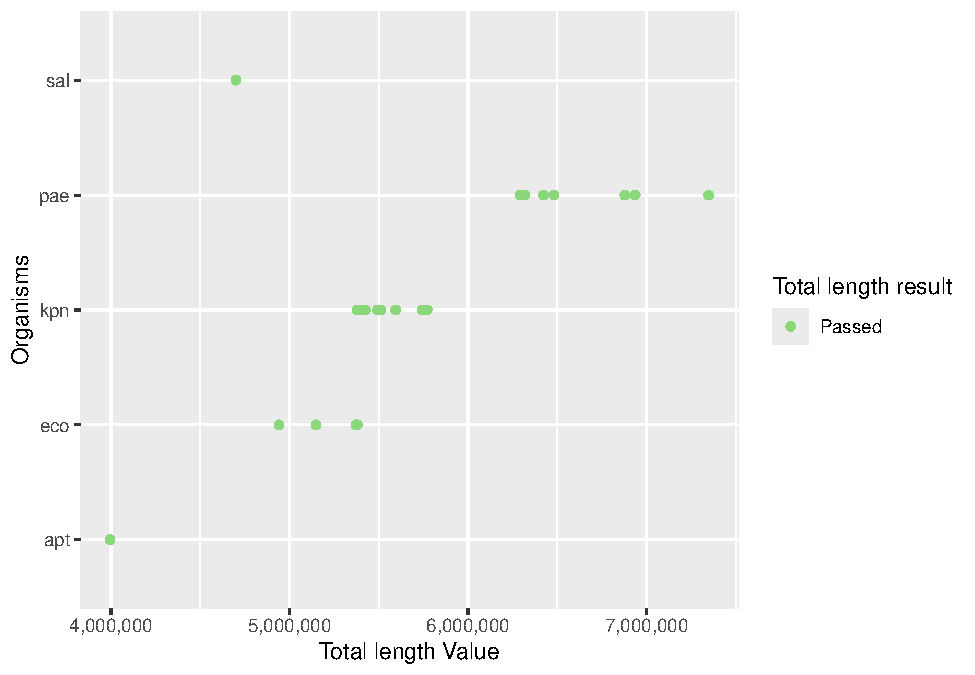
\includegraphics{qualifyr_report_2024-04-07_files/figure-latex/length_result -1.pdf}

\(\\\)

\subsubsection{RECOMMENDATION:}\label{recommendation}

\begin{longtable}[l]{>{\centering\arraybackslash}p{8cm}>{\centering\arraybackslash}p{3cm}>{\centering\arraybackslash}p{4cm}}
\toprule
\cellcolor[HTML]{D4D4D4}{\textbf{Sample ID}} & \cellcolor[HTML]{D4D4D4}{\textbf{Action}} & \cellcolor[HTML]{D4D4D4}{\textbf{Reason}}\\
\midrule
No further action required for this batch. &  & \\
\bottomrule
\end{longtable}

\(\\\)

\subsubsection{MLST RESULTS:}\label{mlst-results}

\begin{longtable}[l]{cccccccccc}
\toprule
\cellcolor[HTML]{D4D4D4}{\textbf{sample\_id}} & \cellcolor[HTML]{D4D4D4}{\textbf{species}} & \cellcolor[HTML]{D4D4D4}{\textbf{MLST}} & \cellcolor[HTML]{D4D4D4}{\textbf{aroC}} & \cellcolor[HTML]{D4D4D4}{\textbf{dnaN}} & \cellcolor[HTML]{D4D4D4}{\textbf{hemD}} & \cellcolor[HTML]{D4D4D4}{\textbf{hisD}} & \cellcolor[HTML]{D4D4D4}{\textbf{purE}} & \cellcolor[HTML]{D4D4D4}{\textbf{sucA}} & \cellcolor[HTML]{D4D4D4}{\textbf{thrA}}\\
\midrule
23ARS\_VSM0511 & Salmonella enterica subsp. enterica serovar Enteritidis & - & 5,638 & 2 & 3 & 7 & 6 & 6 & 11\\
\bottomrule
\end{longtable}
\vspace{1em}
\begin{longtable}[l]{lcccccccccc}
\toprule
\cellcolor[HTML]{D4D4D4}{\textbf{}} & \cellcolor[HTML]{D4D4D4}{\textbf{sample\_id}} & \cellcolor[HTML]{D4D4D4}{\textbf{species}} & \cellcolor[HTML]{D4D4D4}{\textbf{MLST}} & \cellcolor[HTML]{D4D4D4}{\textbf{aroC}} & \cellcolor[HTML]{D4D4D4}{\textbf{dnaN}} & \cellcolor[HTML]{D4D4D4}{\textbf{hemD}} & \cellcolor[HTML]{D4D4D4}{\textbf{hisD}} & \cellcolor[HTML]{D4D4D4}{\textbf{purE}} & \cellcolor[HTML]{D4D4D4}{\textbf{sucA}} & \cellcolor[HTML]{D4D4D4}{\textbf{thrA}}\\
\midrule
2 & 24ARS\_BRH0014 & Pseudomonas aeruginosa & 639 & 11 & 19 & 19 & 3 & 4 & 4 & 7\\
3 & 24ARS\_BRT0017 & Pseudomonas aeruginosa & - & 28,347 & 5 & 36 & 3 & 3 & 13 & 7\\
7 & 24ARS\_DMC0102 & Pseudomonas aeruginosa & 2617 & 84 & 3 & 20 & 71 & 4 & 7 & 1\\
8 & 24ARS\_EVR0011 & Pseudomonas aeruginosa & - & 15,345 & 5 & 11 & 3 & 15 & 42 & 9\\
9 & 24ARS\_EVR0017 & Pseudomonas aeruginosa & 641 & 6 & 5 & 6 & 5 & 4 & 4 & 7\\
\addlinespace
16 & 24ARS\_SLH0030 & Pseudomonas aeruginosa & - & 11,345 & 20 & 1 & 65 & 4 & 4 & 10\\
19 & 24ARS\_ZMC0002 & Pseudomonas aeruginosa & 3014 & 16 & 5 & 12 & 3 & 3 & 1 & 18\\
\bottomrule
\end{longtable}
\vspace{1em}
\begin{longtable}[l]{lcccccccccc}
\toprule
\cellcolor[HTML]{D4D4D4}{\textbf{}} & \cellcolor[HTML]{D4D4D4}{\textbf{sample\_id}} & \cellcolor[HTML]{D4D4D4}{\textbf{species}} & \cellcolor[HTML]{D4D4D4}{\textbf{MLST}} & \cellcolor[HTML]{D4D4D4}{\textbf{aroC}} & \cellcolor[HTML]{D4D4D4}{\textbf{dnaN}} & \cellcolor[HTML]{D4D4D4}{\textbf{hemD}} & \cellcolor[HTML]{D4D4D4}{\textbf{hisD}} & \cellcolor[HTML]{D4D4D4}{\textbf{purE}} & \cellcolor[HTML]{D4D4D4}{\textbf{sucA}} & \cellcolor[HTML]{D4D4D4}{\textbf{thrA}}\\
\midrule
4 & 24ARS\_CRH0017 & Escherichia coli & 2083 & 6 & 322 & 5 & 16 & 11 & 8 & 7\\
13 & 24ARS\_NKI0048 & Escherichia coli & 131 & 53 & 40 & 47 & 13 & 36 & 28 & 29\\
20 & UTP\_ST\_031 & Escherichia coli & 38 & 4 & 26 & 2 & 25 & 5 & 5 & 19\\
\bottomrule
\end{longtable}
\vspace{1em}
\begin{longtable}[l]{lcccccccccc}
\toprule
\cellcolor[HTML]{D4D4D4}{\textbf{}} & \cellcolor[HTML]{D4D4D4}{\textbf{sample\_id}} & \cellcolor[HTML]{D4D4D4}{\textbf{species}} & \cellcolor[HTML]{D4D4D4}{\textbf{MLST}} & \cellcolor[HTML]{D4D4D4}{\textbf{aroC}} & \cellcolor[HTML]{D4D4D4}{\textbf{dnaN}} & \cellcolor[HTML]{D4D4D4}{\textbf{hemD}} & \cellcolor[HTML]{D4D4D4}{\textbf{hisD}} & \cellcolor[HTML]{D4D4D4}{\textbf{purE}} & \cellcolor[HTML]{D4D4D4}{\textbf{sucA}} & \cellcolor[HTML]{D4D4D4}{\textbf{thrA}}\\
\midrule
5 & 24ARS\_CRH0030 & Klebsiella quasipneumoniae & - & 18 & 22 & 74 & 22 & 123 & 20 & 99\\
6 & 24ARS\_DMC0098 & Klebsiella pneumoniae & 17 & 2 & 1 & 1 & 1 & 4 & 4 & 4\\
10 & 24ARS\_GMH0029 & Klebsiella pneumoniae & 147 & 3 & 4 & 6 & 1 & 7 & 4 & 38\\
11 & 24ARS\_JLM0018 & Klebsiella pneumoniae & 39 & 2 & 1 & 2 & 4 & 9 & 1 & 14\\
12 & 24ARS\_JLM0020 & Klebsiella quasipneumoniae & 6403 & 18 & 22 & 26 & 59 & 92 & 13 & 192\\
\addlinespace
14 & 24ARS\_NKI0050 & Klebsiella pneumoniae & 2050 & 2 & 3 & 2 & 37 & 10 & 1 & 15\\
15 & 24ARS\_NKI0051 & Klebsiella pneumoniae & 15 & 1 & 1 & 1 & 1 & 1 & 1 & 1\\
17 & 24ARS\_STU0024 & Klebsiella pneumoniae & 39 & 2 & 1 & 2 & 4 & 9 & 1 & 14\\
\bottomrule
\end{longtable}
\vspace{1em}
\begin{longtable}[l]{lcccccccccc}
\toprule
\cellcolor[HTML]{D4D4D4}{\textbf{}} & \cellcolor[HTML]{D4D4D4}{\textbf{sample\_id}} & \cellcolor[HTML]{D4D4D4}{\textbf{species}} & \cellcolor[HTML]{D4D4D4}{\textbf{MLST}} & \cellcolor[HTML]{D4D4D4}{\textbf{aroC}} & \cellcolor[HTML]{D4D4D4}{\textbf{dnaN}} & \cellcolor[HTML]{D4D4D4}{\textbf{hemD}} & \cellcolor[HTML]{D4D4D4}{\textbf{hisD}} & \cellcolor[HTML]{D4D4D4}{\textbf{purE}} & \cellcolor[HTML]{D4D4D4}{\textbf{sucA}} & \cellcolor[HTML]{D4D4D4}{\textbf{thrA}}\\
\midrule
18 & 24ARS\_STU0027 & Acinetobacter pittii & - & \textasciitilde{}101 & \textasciitilde{}233 & 46 & 29 & \textasciitilde{}124 & \textasciitilde{}59 & 119\\
\bottomrule
\end{longtable}
\vspace{1em}

\(\\\)

\subsubsection{AMR PREDICTION RESULTS:}\label{amr-prediction-results}

\begin{longtable}[l]{ccccccc}
\toprule
\cellcolor[HTML]{D4D4D4}{\textbf{sample\_id}} & \cellcolor[HTML]{D4D4D4}{\textbf{species}} & \cellcolor[HTML]{D4D4D4}{\textbf{AMR EFFLUX}} & \cellcolor[HTML]{D4D4D4}{\textbf{STRESS COPPER/GOLD}} & \cellcolor[HTML]{D4D4D4}{\textbf{STRESS GOLD}} & \cellcolor[HTML]{D4D4D4}{\textbf{STRESS NA}} & \cellcolor[HTML]{D4D4D4}{\textbf{VIRULENCE NA}}\\
\midrule
23ARS\_VSM0511 & Salmonella enterica subsp. enterica serovar Enteritidis & mdsA, mdsB & golT & golS & fieF & sodC1, iroC, iroB, sinH\\
\bottomrule
\end{longtable}
\vspace{1em}
\begin{longtable}[l]{ccccccccccccccccc}
\toprule
\cellcolor[HTML]{D4D4D4}{\textbf{sample\_id}} & \cellcolor[HTML]{D4D4D4}{\textbf{species}} & \cellcolor[HTML]{D4D4D4}{\textbf{AMR AMIKACIN/KANAMYCIN}} & \cellcolor[HTML]{D4D4D4}{\textbf{AMR BETA-LACTAM}} & \cellcolor[HTML]{D4D4D4}{\textbf{AMR CARBAPENEM}} & \cellcolor[HTML]{D4D4D4}{\textbf{AMR CEPHALOSPORIN}} & \cellcolor[HTML]{D4D4D4}{\textbf{AMR CHLORAMPHENICOL}} & \cellcolor[HTML]{D4D4D4}{\textbf{AMR EFFLUX}} & \cellcolor[HTML]{D4D4D4}{\textbf{AMR FOSFOMYCIN}} & \cellcolor[HTML]{D4D4D4}{\textbf{AMR KANAMYCIN}} & \cellcolor[HTML]{D4D4D4}{\textbf{AMR QUINOLONE}} & \cellcolor[HTML]{D4D4D4}{\textbf{AMR STREPTOMYCIN}} & \cellcolor[HTML]{D4D4D4}{\textbf{AMR SULFONAMIDE}} & \cellcolor[HTML]{D4D4D4}{\textbf{AMR TIGECYCLINE}} & \cellcolor[HTML]{D4D4D4}{\textbf{STRESS CHROMATE}} & \cellcolor[HTML]{D4D4D4}{\textbf{STRESS MERCURY}} & \cellcolor[HTML]{D4D4D4}{\textbf{STRESS NA}}\\
\midrule
24ARS\_BRH0014 & Pseudomonas aeruginosa & NA & blaOXA-486 & NA & blaPDC-3 & catB7 & mexA, mexE, mexX & fosA & aph(3')-IIb & NA & NA & NA & NA & NA & NA & NA\\
24ARS\_BRT0017 & Pseudomonas aeruginosa & aph(3')-VIa & blaOXA-396 & blaIMP-26, blaVIM-2 & blaPDC-5, blaOXA-10 & catB7, catB3 & mexA, mexX, mexE & fosA & aph(3')-IIb & qnrVC1 & aadA1, aph(3'')-Ib, aph(3'')-Ib & sul1 & tmexC3, tmexD3, toprJ1 & chrA & merE, merD, merA, merP, merT, merR & clpK\\
24ARS\_DMC0102 & Pseudomonas aeruginosa & NA & blaOXA-486 & NA & blaPDC-5 & catB7 & mexA, mexE, mexX & fosA & aph(3')-IIb & NA & NA & NA & NA & NA & NA & NA\\
24ARS\_EVR0011 & Pseudomonas aeruginosa & NA & blaOXA-50 & NA & blaPDC-3 & catB7 & mexA, mexE, mexX & fosA & aph(3')-IIb & NA & NA & NA & NA & NA & NA & NA\\
24ARS\_EVR0017 & Pseudomonas aeruginosa & NA & blaOXA-50 & NA & blaPDC-5 & catB7 & mexA, mexX, mexE & fosA & aph(3')-IIb & NA & NA & NA & NA & NA & NA & NA\\
\addlinespace
24ARS\_SLH0030 & Pseudomonas aeruginosa & NA & blaOXA-50 & NA & blaPDC-14 & catB7 & mexE, mexA, mexX & fosA & aph(3')-IIb & NA & NA & NA & NA & NA & NA & NA\\
24ARS\_ZMC0002 & Pseudomonas aeruginosa & NA & blaOXA-1023 & NA & blaPDC-3 & catB7 & mexA, mexE, mexX & fosA & aph(3')-IIb & NA & NA & NA & NA & NA & NA & NA\\
\bottomrule
\end{longtable}
\vspace{1em}
\begin{longtable}[l]{cccccccccccccccccccccccc}
\toprule
\cellcolor[HTML]{D4D4D4}{\textbf{sample\_id}} & \cellcolor[HTML]{D4D4D4}{\textbf{species}} & \cellcolor[HTML]{D4D4D4}{\textbf{AMR AMIKACIN/KANAMYCIN/QUINOLONE/TOBRAMYCIN}} & \cellcolor[HTML]{D4D4D4}{\textbf{AMR AZITHROMYCIN/ERYTHROMYCIN/SPIRAMYCIN/TELITHROMYCIN}} & \cellcolor[HTML]{D4D4D4}{\textbf{AMR BETA-LACTAM}} & \cellcolor[HTML]{D4D4D4}{\textbf{AMR BLEOMYCIN}} & \cellcolor[HTML]{D4D4D4}{\textbf{AMR CARBAPENEM}} & \cellcolor[HTML]{D4D4D4}{\textbf{AMR CEPHALOSPORIN}} & \cellcolor[HTML]{D4D4D4}{\textbf{AMR CHLORAMPHENICOL}} & \cellcolor[HTML]{D4D4D4}{\textbf{AMR CLINDAMYCIN/ERYTHROMYCIN}} & \cellcolor[HTML]{D4D4D4}{\textbf{AMR COLISTIN}} & \cellcolor[HTML]{D4D4D4}{\textbf{AMR EFFLUX}} & \cellcolor[HTML]{D4D4D4}{\textbf{AMR GENTAMICIN}} & \cellcolor[HTML]{D4D4D4}{\textbf{AMR KANAMYCIN}} & \cellcolor[HTML]{D4D4D4}{\textbf{AMR STREPTOMYCIN}} & \cellcolor[HTML]{D4D4D4}{\textbf{AMR SULFONAMIDE}} & \cellcolor[HTML]{D4D4D4}{\textbf{AMR TETRACYCLINE}} & \cellcolor[HTML]{D4D4D4}{\textbf{AMR TRIMETHOPRIM}} & \cellcolor[HTML]{D4D4D4}{\textbf{STRESS ARSENATE}} & \cellcolor[HTML]{D4D4D4}{\textbf{STRESS ARSENIC}} & \cellcolor[HTML]{D4D4D4}{\textbf{STRESS EFFLUX}} & \cellcolor[HTML]{D4D4D4}{\textbf{STRESS NA}} & \cellcolor[HTML]{D4D4D4}{\textbf{STRESS QUATERNARY AMMONIUM}} & \cellcolor[HTML]{D4D4D4}{\textbf{VIRULENCE NA}}\\
\midrule
24ARS\_CRH0017 & Escherichia coli & aac(6')-Ib-cr5 & NA & blaEC, blaTEM-1 & ble & blaNDM-7 & blaCMY-42 & catA2 & erm(42) & mcr-1.1 & acrF, mdtM, emrD & aac(3)-IId & aph(3')-Ia & aph(6)-Id, aph(3'')-Ib & sul2 & tet(B) & NA & arsC & arsR & NA & ariR, asr, fieF & NA & fdeC, lpfA-O113, astA, espX1\\
24ARS\_NKI0048 & Escherichia coli & aac(6')-Ib-cr5 & mph(A) & blaEC & NA & NA & blaCTX-M-15, blaOXA-1 & NA & NA & NA & acrF, emrD, mdtM & NA & NA & aadA5 & sul1 & tet(A) & dfrA17 & arsC & NA & emrE & ariR, fieF, asr & qacEdelta1 & fdeC, iss, ybtP, ybtQ, afaC, nfaE, papA, iucA, iucB, iucC, iucD, iutA, sat, iha\\
UTP\_ST\_031 & Escherichia coli & NA & mph(A) & blaEC, blaTEM-1 & NA & NA & blaCTX-M-14 & NA & NA & NA & acrF, emrD & NA & NA & aadA5 & sul1 & NA & dfrA17 & arsC & arsR & NA & asr, fieF, ariR & qacEdelta1 & espX1, fdeC, ybtQ, ybtP, afaC, nfaE, eilA, aap, eatA, astA\\
\bottomrule
\end{longtable}
\vspace{1em}
\begin{longtable}[l]{ccccccccccccccccccccccccccccc}
\toprule
\cellcolor[HTML]{D4D4D4}{\textbf{sample\_id}} & \cellcolor[HTML]{D4D4D4}{\textbf{species}} & \cellcolor[HTML]{D4D4D4}{\textbf{AMR AMIKACIN/KANAMYCIN/QUINOLONE/TOBRAMYCIN}} & \cellcolor[HTML]{D4D4D4}{\textbf{AMR AMINOGLYCOSIDE}} & \cellcolor[HTML]{D4D4D4}{\textbf{AMR AZITHROMYCIN/ERYTHROMYCIN/SPIRAMYCIN/TELITHROMYCIN}} & \cellcolor[HTML]{D4D4D4}{\textbf{AMR BETA-LACTAM}} & \cellcolor[HTML]{D4D4D4}{\textbf{AMR BLEOMYCIN}} & \cellcolor[HTML]{D4D4D4}{\textbf{AMR CARBAPENEM}} & \cellcolor[HTML]{D4D4D4}{\textbf{AMR CEPHALOSPORIN}} & \cellcolor[HTML]{D4D4D4}{\textbf{AMR EFFLUX}} & \cellcolor[HTML]{D4D4D4}{\textbf{AMR FOSFOMYCIN}} & \cellcolor[HTML]{D4D4D4}{\textbf{AMR GENTAMICIN}} & \cellcolor[HTML]{D4D4D4}{\textbf{AMR KANAMYCIN}} & \cellcolor[HTML]{D4D4D4}{\textbf{AMR PHENICOL/QUINOLONE}} & \cellcolor[HTML]{D4D4D4}{\textbf{AMR QUINOLONE}} & \cellcolor[HTML]{D4D4D4}{\textbf{AMR RIFAMYCIN}} & \cellcolor[HTML]{D4D4D4}{\textbf{AMR STREPTOMYCIN}} & \cellcolor[HTML]{D4D4D4}{\textbf{AMR SULFONAMIDE}} & \cellcolor[HTML]{D4D4D4}{\textbf{AMR TETRACYCLINE}} & \cellcolor[HTML]{D4D4D4}{\textbf{AMR TRIMETHOPRIM}} & \cellcolor[HTML]{D4D4D4}{\textbf{STRESS COPPER}} & \cellcolor[HTML]{D4D4D4}{\textbf{STRESS COPPER/SILVER}} & \cellcolor[HTML]{D4D4D4}{\textbf{STRESS MERCURY}} & \cellcolor[HTML]{D4D4D4}{\textbf{STRESS NA}} & \cellcolor[HTML]{D4D4D4}{\textbf{STRESS ORGANOMERCURY}} & \cellcolor[HTML]{D4D4D4}{\textbf{STRESS QUATERNARY AMMONIUM}} & \cellcolor[HTML]{D4D4D4}{\textbf{STRESS SILVER}} & \cellcolor[HTML]{D4D4D4}{\textbf{STRESS TELLURIUM}} & \cellcolor[HTML]{D4D4D4}{\textbf{VIRULENCE NA}}\\
\midrule
24ARS\_CRH0030 & Klebsiella quasipneumoniae & NA & NA & mph(A) & blaOKP-B & NA & NA & blaCTX-M-15 & kdeA, emrD & fosA & NA & NA & oqxA, oqxB & qnrS1 & NA & aadA2, aph(6)-Id, aph(3'')-Ib & sul1, sul2 & tet(A) & dfrA12 & pcoA, pcoB, pcoC, pcoD, pcoR, pcoS & silS, silR, silC, silF, silB, silA & NA & fieF & NA & qacEdelta1 & silE, silP & terB, terC, terD, terE & NA\\
24ARS\_DMC0098 & Klebsiella pneumoniae & aac(6')-Ib-cr5 & NA & mph(A) & blaSHV-11, blaTEM-1 & NA & NA & blaCTX-M-15 & kdeA, emrD & fosA & aac(3)-IId & NA & oqxA, oqxB25 & NA & arr-3 & aadA16 & sul1 & tet(A) & NA & pcoA, pcoB, pcoC, pcoD, pcoR, pcoS & silS, silR, silC, silF, silB, silA & NA & fieF & NA & qacEdelta1 & silE, silP & terB, terC, terD, terE & NA\\
24ARS\_GMH0029 & Klebsiella pneumoniae & aac(6')-Ib-cr & rmtB1 & mph(A) & blaSHV-11 & ble & blaNDM-7 & blaCTX-M-15, blaOXA-1 & kdeA, emrD & fosA & aac(3)-IIe & NA & oqxA, oqxB & qnrB6 & arr-3 & aadA16 & sul1 & tet(A) & NA & NA & NA & NA & fieF & NA & qacEdelta1 & NA & NA & NA\\
24ARS\_JLM0018 & Klebsiella pneumoniae & aac(6')-Ib-cr5 & NA & mph(A) & blaSHV-11 & ble & blaNDM-5 & blaCTX-M-15, blaOXA-1 & kdeA, emrD & fosA & aac(3)-IId & NA & oqxA, oqxB32 & qnrS1, qnrB6 & arr-3 & aadA16, aadA2, aph(3'')-Ib & sul1 & tet(A) & dfrA12 & pcoA, pcoB, pcoC, pcoD, pcoR, pcoS & silS, silR, silC, silF, silB, silA & merP, merT, merR & fieF & merC & NA & silE, silP & terB, terC, terD, terE & ybtP, ybtQ\\
24ARS\_JLM0020 & Klebsiella quasipneumoniae & NA & NA & mph(A) & blaOKP-B & NA & NA & blaCTX-M-15 & emrD, kdeA & fosA & NA & NA & oqxA, oqxB & qnrS1 & NA & aadA2, aph(3'')-Ib, aph(6)-Id & sul1, sul2 & tet(A) & dfrA12 & pcoS, pcoR, pcoD, pcoC, pcoB, pcoA & silA, silB, silF, silC, silR, silS & NA & fieF & NA & qacEdelta1 & silP, silE & terB, terC, terD, terE & NA\\
\addlinespace
24ARS\_NKI0050 & Klebsiella pneumoniae & NA & NA & NA & blaSHV-1 & NA & NA & NA & emrD, kdeA & fosA & NA & NA & oqxA, oqxB25 & NA & NA & NA & NA & NA & NA & pcoA, pcoB, pcoC, pcoD, pcoR, pcoS & silS, silR, silC, silF, silB, silA & NA & fieF & NA & NA & silE, silP & terE, terD, terC, terB & ybtQ, ybtP, iroB, iroC, iroD, iroN, peg-344, rmpC, rmpA, iutA, iucC, iucB, iucA\\
24ARS\_NKI0051 & Klebsiella pneumoniae & aac(6')-Ib-cr5 & NA & mph(A) & blaSHV-28 & ble & blaNDM-5 & blaCTX-M-15, blaOXA-1 & emrD, kdeA & fosA & aac(3)-IIe & NA & oqxA, oqxB & qnrS1, qnrB1 & NA & aadA2, aph(6)-Id, aph(3'')-Ib & sul1, sul2 & NA & dfrA12 & pcoA, pcoB, pcoC, pcoD, pcoR, pcoS & silS, silR, silC, silF, silB, silA & NA & fieF & NA & qacEdelta1 & silE, silP & terB, terC, terD, terE & NA\\
24ARS\_STU0024 & Klebsiella pneumoniae & NA & NA & NA & blaSHV-11 & NA & NA & blaCTX-M-15 & kdeA, emrD & fosA & NA & aph(3')-Ia & oqxA, oqxB32 & qnrS1 & NA & aph(3'')-Ib, aph(6)-Id & sul2, sul1 & NA & dfrA7 & pcoA, pcoB, pcoC, pcoD, pcoR, pcoS & silS, silR, silC, silF, silB, silA & NA & fieF & NA & qacEdelta1 & silE, silP & terB, terC, terD, terE & ybtQ, ybtP\\
\bottomrule
\end{longtable}
\vspace{1em}
\begin{longtable}[l]{cccccccc}
\toprule
\cellcolor[HTML]{D4D4D4}{\textbf{sample\_id}} & \cellcolor[HTML]{D4D4D4}{\textbf{species}} & \cellcolor[HTML]{D4D4D4}{\textbf{AMR CARBAPENEM}} & \cellcolor[HTML]{D4D4D4}{\textbf{AMR CEPHALOSPORIN}} & \cellcolor[HTML]{D4D4D4}{\textbf{AMR EFFLUX}} & \cellcolor[HTML]{D4D4D4}{\textbf{AMR FOSFOMYCIN}} & \cellcolor[HTML]{D4D4D4}{\textbf{AMR SPECTINOMYCIN/STREPTOMYCIN}} & \cellcolor[HTML]{D4D4D4}{\textbf{STRESS NICKEL}}\\
\midrule
24ARS\_STU0027 & Acinetobacter pittii & blaOXA & blaADC & amvA, adeE, adeD & abaF & ant(3'')-IIa & nreB\\
\bottomrule
\end{longtable}
\vspace{1em}

\begin{table}
\centering\begingroup\fontsize{7}{9}\selectfont

\begin{tabular}{l>{\raggedright\arraybackslash}p{1cm}>{\raggedright\arraybackslash}p{1cm}>{\raggedright\arraybackslash}p{1cm}>{\raggedright\arraybackslash}p{1cm}>{\raggedright\arraybackslash}p{1cm}>{\raggedright\arraybackslash}p{1cm}>{\raggedright\arraybackslash}p{1cm}>{\raggedright\arraybackslash}p{1cm}>{\raggedright\arraybackslash}p{1cm}>{\raggedright\arraybackslash}p{1cm}>{\raggedright\arraybackslash}p{1cm}>{\raggedright\arraybackslash}p{1cm}>{\raggedright\arraybackslash}p{1cm}>{\raggedright\arraybackslash}p{1cm}>{\raggedright\arraybackslash}p{1cm}>{\raggedright\arraybackslash}p{1cm}>{\raggedright\arraybackslash}p{1cm}>{\raggedright\arraybackslash}p{1cm}>{\raggedright\arraybackslash}p{1cm}>{\raggedright\arraybackslash}p{1cm}>{\raggedright\arraybackslash}p{1cm}>{\raggedright\arraybackslash}p{1cm}>{\raggedright\arraybackslash}p{1cm}>{\raggedright\arraybackslash}p{1cm}>{\raggedright\arraybackslash}p{1cm}>{\raggedright\arraybackslash}p{1cm}>{\raggedright\arraybackslash}p{1cm}>{\raggedright\arraybackslash}p{1cm}}
\toprule
sample\_id & species & AMR AMIKACIN/KANAMYCIN/QUINOLONE/TOBRAMYCIN & AMR AMINOGLYCOSIDE & AMR AZITHROMYCIN/ERYTHROMYCIN/SPIRAMYCIN/TELITHROMYCIN & AMR BETA-LACTAM & AMR BLEOMYCIN & AMR CARBAPENEM & AMR CEPHALOSPORIN & AMR EFFLUX & AMR FOSFOMYCIN & AMR GENTAMICIN & AMR KANAMYCIN & AMR PHENICOL/QUINOLONE & AMR QUINOLONE & AMR RIFAMYCIN & AMR STREPTOMYCIN & AMR SULFONAMIDE & AMR TETRACYCLINE & AMR TRIMETHOPRIM & STRESS COPPER & STRESS COPPER/SILVER & STRESS MERCURY & STRESS NA & STRESS ORGANOMERCURY & STRESS QUATERNARY AMMONIUM & STRESS SILVER & STRESS TELLURIUM & VIRULENCE NA\\
\midrule
24ARS\_CRH0030 & Klebsiella quasipneumoniae & NA & NA & mph(A) & blaOKP-B & NA & NA & blaCTX-M-15 & kdeA, emrD & fosA & NA & NA & oqxA, oqxB & qnrS1 & NA & aadA2, aph(6)-Id, aph(3'')-Ib & sul1, sul2 & tet(A) & dfrA12 & pcoA, pcoB, pcoC, pcoD, pcoR, pcoS & silS, silR, silC, silF, silB, silA & NA & fieF & NA & qacEdelta1 & silE, silP & terB, terC, terD, terE & NA\\
24ARS\_DMC0098 & Klebsiella pneumoniae & aac(6')-Ib-cr5 & NA & mph(A) & blaSHV-11, blaTEM-1 & NA & NA & blaCTX-M-15 & kdeA, emrD & fosA & aac(3)-IId & NA & oqxA, oqxB25 & NA & arr-3 & aadA16 & sul1 & tet(A) & NA & pcoA, pcoB, pcoC, pcoD, pcoR, pcoS & silS, silR, silC, silF, silB, silA & NA & fieF & NA & qacEdelta1 & silE, silP & terB, terC, terD, terE & NA\\
24ARS\_GMH0029 & Klebsiella pneumoniae & aac(6')-Ib-cr & rmtB1 & mph(A) & blaSHV-11 & ble & blaNDM-7 & blaCTX-M-15, blaOXA-1 & kdeA, emrD & fosA & aac(3)-IIe & NA & oqxA, oqxB & qnrB6 & arr-3 & aadA16 & sul1 & tet(A) & NA & NA & NA & NA & fieF & NA & qacEdelta1 & NA & NA & NA\\
24ARS\_JLM0018 & Klebsiella pneumoniae & aac(6')-Ib-cr5 & NA & mph(A) & blaSHV-11 & ble & blaNDM-5 & blaCTX-M-15, blaOXA-1 & kdeA, emrD & fosA & aac(3)-IId & NA & oqxA, oqxB32 & qnrS1, qnrB6 & arr-3 & aadA16, aadA2, aph(3'')-Ib & sul1 & tet(A) & dfrA12 & pcoA, pcoB, pcoC, pcoD, pcoR, pcoS & silS, silR, silC, silF, silB, silA & merP, merT, merR & fieF & merC & NA & silE, silP & terB, terC, terD, terE & ybtP, ybtQ\\
24ARS\_JLM0020 & Klebsiella quasipneumoniae & NA & NA & mph(A) & blaOKP-B & NA & NA & blaCTX-M-15 & emrD, kdeA & fosA & NA & NA & oqxA, oqxB & qnrS1 & NA & aadA2, aph(3'')-Ib, aph(6)-Id & sul1, sul2 & tet(A) & dfrA12 & pcoS, pcoR, pcoD, pcoC, pcoB, pcoA & silA, silB, silF, silC, silR, silS & NA & fieF & NA & qacEdelta1 & silP, silE & terB, terC, terD, terE & NA\\
\addlinespace
24ARS\_NKI0050 & Klebsiella pneumoniae & NA & NA & NA & blaSHV-1 & NA & NA & NA & emrD, kdeA & fosA & NA & NA & oqxA, oqxB25 & NA & NA & NA & NA & NA & NA & pcoA, pcoB, pcoC, pcoD, pcoR, pcoS & silS, silR, silC, silF, silB, silA & NA & fieF & NA & NA & silE, silP & terE, terD, terC, terB & ybtQ, ybtP, iroB, iroC, iroD, iroN, peg-344, rmpC, rmpA, iutA, iucC, iucB, iucA\\
24ARS\_NKI0051 & Klebsiella pneumoniae & aac(6')-Ib-cr5 & NA & mph(A) & blaSHV-28 & ble & blaNDM-5 & blaCTX-M-15, blaOXA-1 & emrD, kdeA & fosA & aac(3)-IIe & NA & oqxA, oqxB & qnrS1, qnrB1 & NA & aadA2, aph(6)-Id, aph(3'')-Ib & sul1, sul2 & NA & dfrA12 & pcoA, pcoB, pcoC, pcoD, pcoR, pcoS & silS, silR, silC, silF, silB, silA & NA & fieF & NA & qacEdelta1 & silE, silP & terB, terC, terD, terE & NA\\
24ARS\_STU0024 & Klebsiella pneumoniae & NA & NA & NA & blaSHV-11 & NA & NA & blaCTX-M-15 & kdeA, emrD & fosA & NA & aph(3')-Ia & oqxA, oqxB32 & qnrS1 & NA & aph(3'')-Ib, aph(6)-Id & sul2, sul1 & NA & dfrA7 & pcoA, pcoB, pcoC, pcoD, pcoR, pcoS & silS, silR, silC, silF, silB, silA & NA & fieF & NA & qacEdelta1 & silE, silP & terB, terC, terD, terE & ybtQ, ybtP\\
\bottomrule
\end{tabular}
\endgroup{}
\end{table}

\end{document}
